\documentclass{ximera}


\graphicspath{
  {./}
  {ximeraTutorial/}
  {basicPhilosophy/}
}

\newcommand{\mooculus}{\textsf{\textbf{MOOC}\textnormal{\textsf{ULUS}}}}

\usepackage{tkz-euclide}\usepackage{tikz}
\usepackage{tikz-cd}
\usetikzlibrary{arrows}
\tikzset{>=stealth,commutative diagrams/.cd,
  arrow style=tikz,diagrams={>=stealth}} %% cool arrow head
\tikzset{shorten <>/.style={ shorten >=#1, shorten <=#1 } } %% allows shorter vectors

\usetikzlibrary{backgrounds} %% for boxes around graphs
\usetikzlibrary{shapes,positioning}  %% Clouds and stars
\usetikzlibrary{matrix} %% for matrix
\usepgfplotslibrary{polar} %% for polar plots
\usepgfplotslibrary{fillbetween} %% to shade area between curves in TikZ
\usetkzobj{all}
\usepackage[makeroom]{cancel} %% for strike outs
%\usepackage{mathtools} %% for pretty underbrace % Breaks Ximera
%\usepackage{multicol}
\usepackage{pgffor} %% required for integral for loops



%% http://tex.stackexchange.com/questions/66490/drawing-a-tikz-arc-specifying-the-center
%% Draws beach ball
\tikzset{pics/carc/.style args={#1:#2:#3}{code={\draw[pic actions] (#1:#3) arc(#1:#2:#3);}}}



\usepackage{array}
\setlength{\extrarowheight}{+.1cm}
\newdimen\digitwidth
\settowidth\digitwidth{9}
\def\divrule#1#2{
\noalign{\moveright#1\digitwidth
\vbox{\hrule width#2\digitwidth}}}






\DeclareMathOperator{\arccot}{arccot}
\DeclareMathOperator{\arcsec}{arcsec}
\DeclareMathOperator{\arccsc}{arccsc}

















%%This is to help with formatting on future title pages.
\newenvironment{sectionOutcomes}{}{}


\author{Lee Wayand}

\begin{document}
\begin{exercise}  





Below is the graph of $y=B(t)$.  

\begin{image}
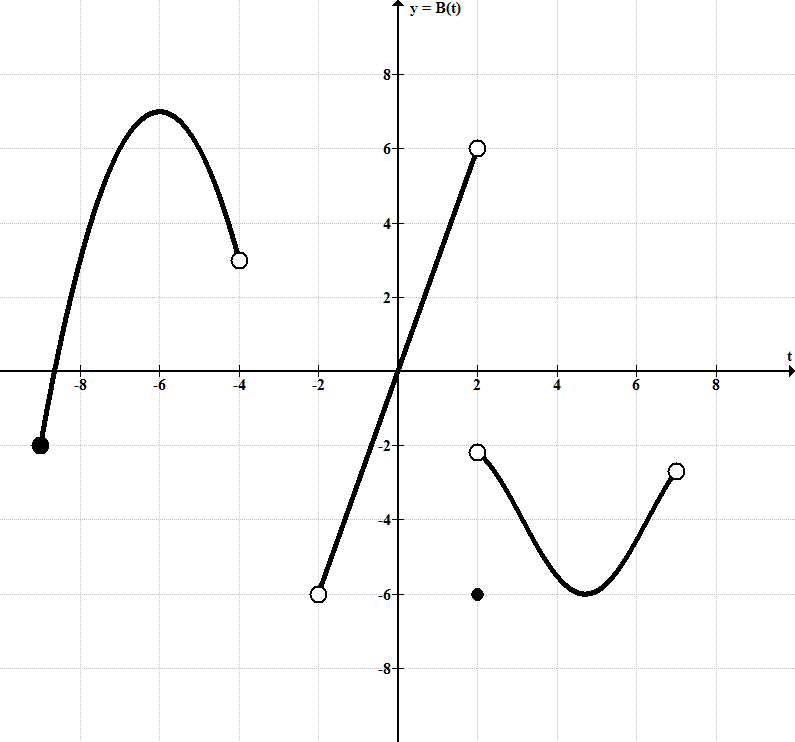
\includegraphics{../../pics/func_graphs/f23.png}
\end{image}


The domain of $f$ is $[-9, -4) \cup (-2, 7)$.\\






\begin{question} 


Evaluate $B(2) = \answer[tolerance=0.25]{-6}$



Classify $2$. \\


\begin{multipleChoice}
\choice [correct]{Discontinuity}
\choice {Singularity}
\choice {Neither}
\end{multipleChoice}







Classify $-4$. \\


\begin{multipleChoice}
\choice {Discontinuity}
\choice {Singularity}
\choice [correct]{Neither}
\end{multipleChoice}






Classify $-2$. \\


\begin{multipleChoice}
\choice {Discontinuity}
\choice {Singularity}
\choice [correct]{Neither}
\end{multipleChoice}




Classify $7$. \\


\begin{multipleChoice}
\choice {Discontinuity}
\choice {Singularity}
\choice [correct]{Neither}
\end{multipleChoice}




\end{question}










\begin{question} 


$(-6, 7)$ is a global maximum of $B$. \\


\begin{multipleChoice}
\choice {True}
\choice [correct]{False}
\end{multipleChoice}




$(2, -6)$ is a global minimum of $B$. \\


\begin{multipleChoice}
\choice {True}
\choice [correct]{False}
\end{multipleChoice}

\end{question}






\begin{question} 



$-6$ is a global minimum, which occurs how many times.


\begin{multipleChoice}
\choice {$0$}
\choice {$1$}
\choice [correct]{$2$}
\choice {$3$}
\choice {$4$}
\end{multipleChoice}


\end{question}





\begin{question} 

There exists a real number, $M$, such that $B(t) < M$ for all $t$ in the domain.
\begin{multipleChoice}
\choice [correct]{True}
\choice {False}
\end{multipleChoice}

\end{question}







\begin{question} 

For any $\epsilon > 0$, there exists a domain number in the interval $(-9-\epsilon, -9+\epsilon)$.
\begin{multipleChoice}
\choice [correct]{True}
\choice {False}
\end{multipleChoice}


\end{question}









\begin{question} 

For any $\epsilon > 0$, there exists a domain number, $d$, in the interval $(2-\epsilon, 2+\epsilon)$ such that $B(d) > 4$.
\begin{multipleChoice}
\choice [correct]{True}
\choice {False}
\end{multipleChoice}


\end{question}







\begin{question} 


The equation $B(t) = 0$ has $\answer{2}$ solutions. \\


The equation $B(t) = 4$ has $\answer{3}$ solutions. \\


The equation $B(t) = 8$ has $\answer{0}$ solutions. \\


The equation $B(t) = -4$ has $\answer{3}$ solutions. \\


The equation $B(t) = -5$ has $\answer{3}$ solutions. \\


The equation $B(t) = -2$ has $\answer{2}$ solutions. \\


\end{question}







\end{exercise}
\end{document}